


% This LaTeX was auto-generated from an M-file by MATLAB.
% To make changes, update the M-file and republish this document.






  
    

\section{Morgenstern Price Slice Tester} \label{sec:MPTests}
Testing results obtained from the MorgPriceSolver.m program, a module in
the SSA program. Factor of safety results from the program are
compared to results from examples in slope stability papers, to judge the
accuracy of the implemented algorithm. Due to the comparison analysis of
the slip surfaces being imperfect definitive pass or fail assessments are
not used, so results are measured on a relative and objective scale. The
general rule of less relative error between results and comparisons
suggests a more accurate solution can be used. For the same slip the
result may be more accurate towards some comparisons more than others. In
these cases ...?? . As a guideline relative error less than 10\% could be
considered acceptable, less than 5\% good, and less than 1\% excellent.

\subsection{Fredlund and Krahn (1977)}
Results compared to the Fredlund and Krahn (1977) paper. A graph of the
relative error between the factor of safety calculated by the program
with the factor of safety given in the paper, as a function of the number
of analysis slices is used to analyze the results. For this paper a
circular and non circular slip surface for the same slope are studied,
under both dry and wet conditions.


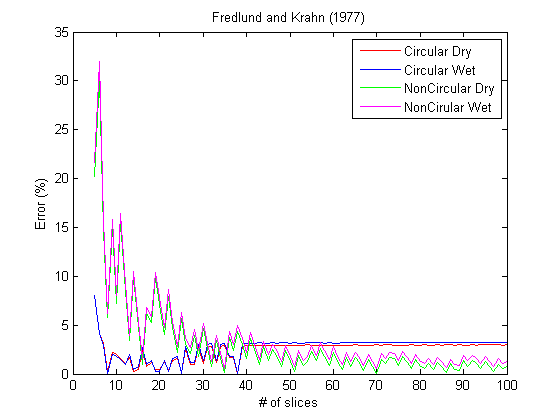
\includegraphics [width=5in]{./VV_SubDocuments/MPSliceTester_01.png}



The figure shows very large error at low numbers of slices, up until
approximately 20 slice analysis. Accuracy then begins to level off and
stays consistent. The graph also shows that the dry analysis has less
relative error than the wet analysis for both circular and non circular
analysis. It can also be seen that the circular slip converges to less
relative error than the non circular analysis. This suggests that the
simpler dry and circular cases produce more accurate results, however
further analysis of this type would be needed for a concrete conclusion.

~\newline \noindent
Inspecting the computation of the factor of safety at extremely large
numbers of slices shows no noticeable change in the returned value.
Convergence to the same factor of safety occurs at 100 and 100000
slices, as seen on the following graph.


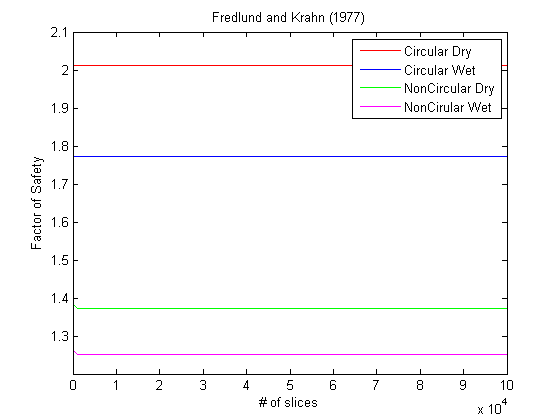
\includegraphics [width=5in]{./VV_SubDocuments/MPSliceTester_02.png}



The next graph shows the change in computation time for calculation of
the slope with different slice numbers. An approximately linear increase
in computation time with number of analysis slices can be seen. As using
a large number of slices sees no noticeable increase in the calculation
of the Factor of Safety, the increased computation time makes using more
slices than approximately 50 unnecessary. When compared to the 
computation time results the RFEM solver (\ref{sec:RFEMTests}), it can be 
seen that the computation time for the morgenstern price algorithm is 
significantly less.


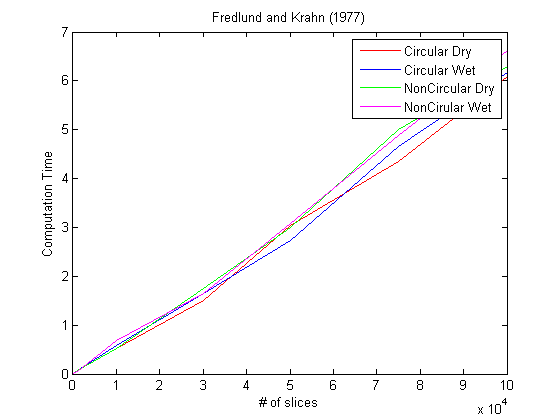
\includegraphics [width=5in]{./VV_SubDocuments/MPSliceTester_03.png}



\subsection{Examples 1 - 5}
Results from the examples used in the papers: Greco (1996), Malkawi et al
(2001) Zolfaghari et al (2005), Sarma and Tan (2006), Pham and Fredlund
(2003), Cheng et al (2007), and Li et al (2010). Results followed the
same general pattern as the previous test: Converging to a consistent
factor of safety at approximately 25 slices. Relative error between
results achieved and the results from the examples in the papers are all
less than 10\%, and for some lower than 1\%. For examples with multiple
comparisons the result usually converges very strongly to at least one
of the comparisons. It should again be noted that the accuracy of results
is relative only to the accuracy of the results from the comparison
papers. However consistently high accuracy compared to results from
different papers in many different examples, means a large true error
would suggest a flaw in the slope stability analysis community as a
whole. Not displayed here, but it was also seen that a large number of
slices resulted in no noticeable change in the factor of safety
calculation.


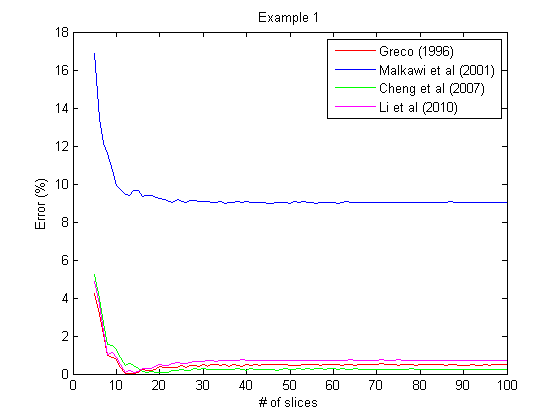
\includegraphics [width=5in]{./VV_SubDocuments/MPSliceTester_04.png}




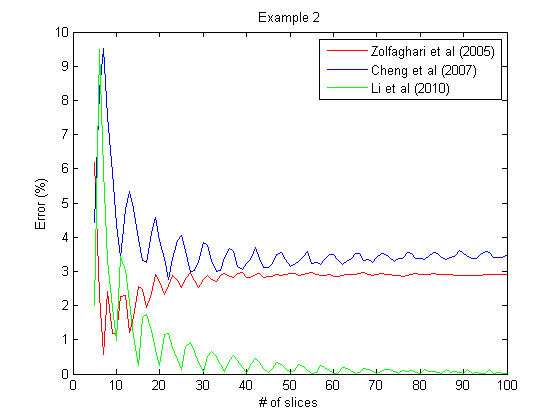
\includegraphics [width=5in]{./VV_SubDocuments/MPSliceTester_05.png}




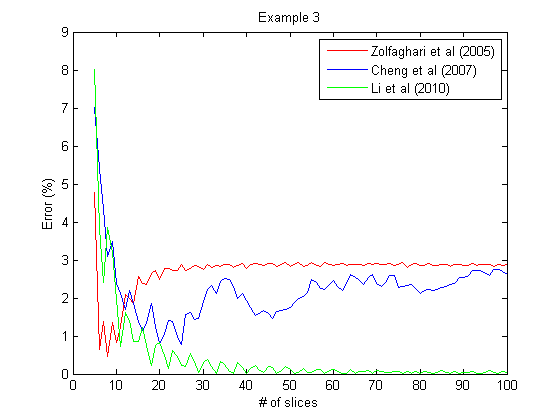
\includegraphics [width=5in]{./VV_SubDocuments/MPSliceTester_06.png}




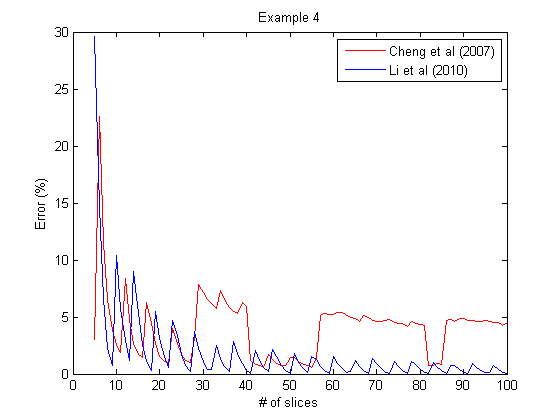
\includegraphics [width=5in]{./VV_SubDocuments/MPSliceTester_07.png}




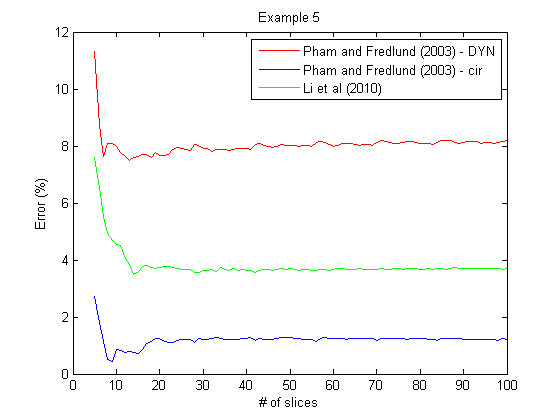
\includegraphics [width=5in]{./VV_SubDocuments/MPSliceTester_08.png}



\subsection{Example 6}
Results from the example used in the papers: Pham and Fredlund (2003), Li
et al (2010). Analysis of this example demonstrated non convergence of
the Factor of Safety calculation for specific slice counts of the
circular Pham and Fredlund analysis. Non convergence occurs when the
algorithm calculates a very low factor of safety, or if the algorithm
solution doesn't become consistent within the limited amount of
iterations.


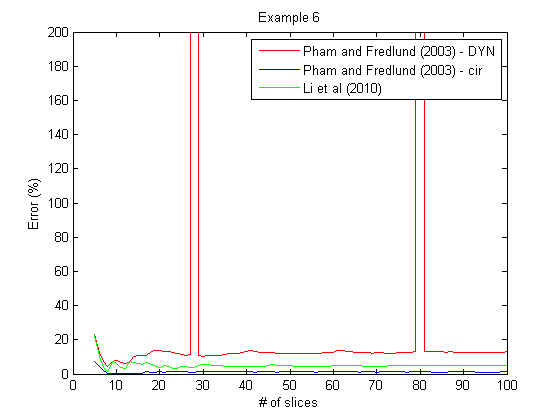
\includegraphics [width=5in]{./VV_SubDocuments/MPSliceTester_09.png}



As a special case the limiting number of iterations allowed for the
analysis was raised from 20 iterations to 30. The previously non
converging results now converge to approximately 15% error, as can be
seen in the following figure. This is less accurate than the results seen
previously, which were generally under 10%. This demonstrates the trade
off between raising the iteration limit allowing better convergence, but
decreasing the overall accuracy of the solver.

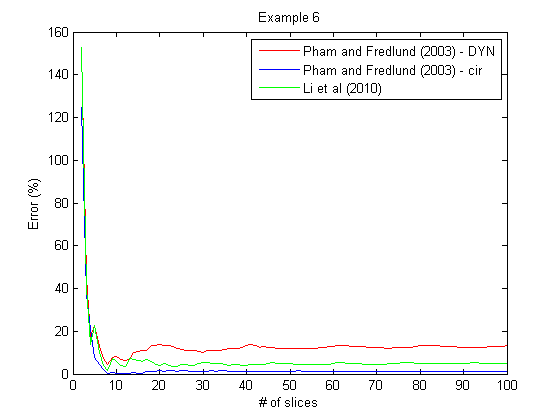
\includegraphics[width=5in]{./VV_SubDocuments/MPSlice_SpecialCase.png}
